\documentclass{standalone}

% Plotting
\usepackage{tikz}
\usetikzlibrary{decorations.markings}
\usetikzlibrary{calc}
% quantikz breaks tikz-cd, see https://tex.stackexchange.com/questions/618330/quantikz-breaks-spacing-in-tikz-matrices-tikz-cd
%\usetikzlibrary{quantikz}
\usetikzlibrary{cd}
\usepackage{pgfplots}

\usepackage{simpler-wick}
\usepackage{physics}

\usepackage{amsmath}
\usepackage{mathtools}

\begin{document}
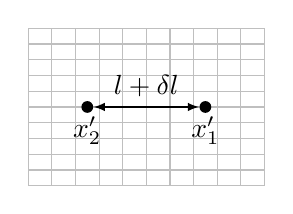
\begin{tikzpicture}[xscale=1.5]
    \foreach \i in {-0.5,-0.3,...,1.5} {
        \draw[lightgray] (\i,-1) -- (\i,1);
    }

    \foreach \i in {-1,-0.8,...,1} {
        \draw[lightgray] (-0.5,\i) -- (1.5,\i);
    }
    \node (x2) at (0,0) [circle,fill,inner sep=1.5pt]{};
    \node (x1) at (1,0) [circle,fill,inner sep=1.5pt]{};

    \draw (x1) node[below] {$x'_1$};
    \draw (x2) node[below] {$x'_2$};
    
    \draw[latex-latex] (x1) -- (x2) node[midway, above] {$l+\delta l$};
\end{tikzpicture}
\end{document}